%%%%%%%%%%%%%%%%%%%%%%%%%%%%%%%%%%%%
% This is the template for submission to HPCA 2018
% The cls file is a modified from  'sig-alternate.cls'
%%%%%%%%%%%%%%%%%%%%%%%%%%%%%%%%%%%%

\documentclass{sig-alternate}
\setlength{\paperheight}{11in}
\setlength{\paperwidth}{8.5in}

\newcommand{\ignore}[1]{}
\usepackage[pass]{geometry}
\usepackage{fancyhdr}
\usepackage[normalem]{ulem}
\usepackage[hyphens]{url}
\usepackage{hyperref}
\usepackage{amsmath}
\usepackage{bookmark}




%%%%%%%%%%%---SETME-----%%%%%%%%%%%%%
\newcommand{\hpcasubmissionnumber}{XXX}
%%%%%%%%%%%%%%%%%%%%%%%%%%%%%%%%%%%%

\fancypagestyle{firstpage}{
  \fancyhf{}
\setlength{\headheight}{50pt}
\renewcommand{\headrulewidth}{0pt}
  \fancyhead[C]{\normalsize{HPCA 2019 Submission
      \textbf{\#\hpcasubmissionnumber} -- Confidential Draft -- Do NOT Distribute!!}}
  \pagenumbering{arabic}
}

%%%%%%%%%%%---SETME-----%%%%%%%%%%%%%
\title{Resource and Runtime Efficiency for Multi Fibonacci Algorithm}
\author{}
%%%%%%%%%%%%%%%%%%%%%%%%%%%%%%%%%%%%

\begin{document}
\maketitle
\thispagestyle{firstpage}
\pagestyle{plain}



%%%%%% -- PAPER CONTENT STARTS-- %%%%%%%%

\begin{abstract}

The need for speed with respect to processing large data sets and the ability to optimize an algorithm allow for more efficient programming. This investigation explores and compares runtime efficiency and resource consumption for both recursive and dynamic programming across several different programming languages that abstract widely differing architectural elements. Utilizing the Fibonacci algorithm, we show that compiled languages demonstrated significantly better runtime efficiency than the interpreted languages studied. However, when an interpreted language is optimized with, for example, a decorator function, its execution time is comparable to that of other compiled languages. An example of this is the interpreted language, Python. Compared to C, a compiled language, the decorated Python algorithm was almost 90 times faster than C when recursively calculating the 40th index of the Fibonacci sequence. Concurrently, the results indicated that the interpreted languages required more computational resource in pursuit of this faster execution time. In addition, comparing a compiled language to an interpreted language with no optimizations yielded different results. Compared to Python, which is interpreted, Go executed the recursive algorithm, on average, 1267.44\% faster, but 1395.18\% slower for the dynamic algorithm. The results also indicated that the compiled languages required more computational resources in pursuit of this faster execution. A full comparison of all studied languages is presented, the potential factors behind the results analyzed, and the possible ramifications for applicable use cases discussed.

\end{abstract}

\section{Introduction}
Algorithmic efficiency has become hugely important due to the need to analyze massive data sets generated by cloud computing and the Internet of Things. While making algorithms more succinct and comprehensive, recursion can also be highly inefficient when applied to these data sets. As an alternative to recursion in many applications, dynamic programming techniques can significantly improve runtime efficiency. Although runtime efficiency has been widely studied for specific problem applications, less attention has been given to the relationship of language and underlying architecture to a broader measure of efficiency that includes both runtime and resource consumption.

Different programming languages are utilized for different purposes, which leads to the question of when to use one language over another? Compiled languages utilize a compiler to take the whole program as input and compile it only once. They generally execute faster than interpreted languages and take up more memory to create the object code as output [1]. Interpreted languages utilize an interpreter, which reads in a single line of code at a time. Because the syntax tree is processed directly to evaluate or execute statements, some of the code may be processed over and over again, resulting in slower execution for interpreted languages [1]. Some common examples of compiled languages include C and Go. Common examples of interpreted languages include Python and Perl. 

This paper presents comparisons between several different programming languages, to include interpreted and compiled, and analyzes their performance efficiencies. As a way to make Python more comparable to the compiled language of C, ways of code optimization were explored. As a result, a version of inline C and a Python implementation with a decorator function to store the results needed later for computation were tested.

\section{Background}

In this section, there will be a list of several key concepts and formulas relevant to this research. While this work focuses mainly on C and Python, the generalizations mentioned can be applied to the general concept of compiled languages as opposed to interpreted languages. 

\subsection{Programming Languages}	

We utilized four languages in our study:

\begin{enumerate}
\item {\em}C is a compiled language created in 1972 at Bell Labs for UNIX system implementation [1]. C is the basis of the programming languages of Java and C++. It is often chosen when speed is a priority for inputs consisting of large data sets [2]. Although it isn't the most simple language to develop with, it is a major player in High Performance Computing (HPC) because of its efficiency in performance [3].
\item {\em}Go is a relatively new programming language created by Google. Go is useful for systems programming and scalable network servers. It is a close second behind C when it comes to speed, and is a relatively simple language to develop with [3]. It is based upon C's implementation; however, it was developed with a focus on a simpler design for the programmer [3]. 
\item {\em}Python is an interpreted language created in 1991 [4]. It has recently made a presence in the HPC world through its packages, such as NumPy, SciPy, and scikit-learn; with these packages, Python applications are optimized to take full 
advantage of the present architecture [4]. With such a presence in HPC, it is clear that Python is here to stay.
\item  {\em}Perl is a common scripting language that utilizes an interpreter. Like Python, it too, has a large variety of libraries to pull from. Perl is quicker and more efficient than Python in term of input/output operations [5]. In addition, Perl is a useful language due to it having a large number of parallel computing modules available.
\end{enumerate}


\subsection{Decorated Python}

As a way to make Python more comparable to the execution speed of C, a decorator function with a wrapper was implemented. Decorator functions are more commonly utilized for tracing, locking, or logging [6]. However, a decorator function combined with a Python wrapper can also be created as a way to make a program more dynamic by having it remember the results needed later for computation. This allowed its performance to be much more comparable to that of the compiled languages in terms of execution time.

\subsection{Inline C}

A method to optimize C was also explored utilizing the keyword ''inline'' before the function call. Inline is a useful tool with smaller functions that will be called multiple times in order to reduce function overhead. Utilizing the inline keyword reduces function call overhead by replacing the actual call with the contents of the function itself. Because of this replacement of the function call with the function contents, it is not very useful with multiple recursive calls as there will be a tradeoff in terms of instruction count and efficiency.

\section{Experimental Methodology}

In the following subsections, different aspects of the study will be described. This will include the initialization of the environment, the execution, the analysis, and the results.

\subsection{Environment}

In this subsection, the elements used to set up the environment are described. We used an Intel NUC NUC5CPYH with the Intel Celeron processor up to 2.48 GHz, with Ubuntu 16.04 installed, a gcc version of 5.4.0, and python 2.7. We installed the other necessary languages for the experiment, so that the NUC had Perl, Python, C, and Go installed. We also installed perf, a resource monitoring utility, so that we could monitor the resource consumption of the different languages. 

\subsection{Execution}

The Fibonacci algorithm gathered from Rosetta Code was utilized as the testing algorithm [8]. Rosetta Code is a repository which contains different algorithms with many programming languages to choose from. A recursive and dynamic version of the Fibonacci algorithm was used from this site for the testing algorithm. Fibonacci values of 20, 30, 40, and 50 were used as function parameters for testing purposes.

\subsection{Analysis}

A profile monitoring resource was used to monitor the resource consumption of the algorithms in order to collect data. Perf is a sample based Linux profiler which monitors Linux perf events [9]. It was utilized for every trial, testing task-clock, CPU-cycles, instruction count, the number of CPUs utilized, clock rate, instructions per second, elapsed time, page-faults, cache-misses, and percent of all cache references. Perf is a sample based profiler. This means that it only uses part of the runtime to get data for the desired perf event, and is commonly used in research. The time command was also used to calculate the time sum consisting of user and system time. Speedup was calculated using the execution times between the different languages.

\section{Results}

The results for this section are split-up according to algorithm results, programming language results, and optimized programming language results. The optimized language results will include the inline C and decorated Python result explanations.

\subsection{Algorithm Results}

The overall runtime for the recursive algorithms were larger than the dynamic algorithm runtimes. The general trend for the recursive algorithms included an increase in resource consumption for the Fibonacci numbers of 30 and 40, whereas the dynamic algorithm results trended mostly linearly. Because of the characteristics of recursive algorithms, it is expected for the runtimes to be slower as there is higher overhead from the call stack being used so heavily. Furthermore, programs are bounded by physical memory, so it is likely that Perl, Python, and Go reached their limit. Otherwise, as the compiler was setting up the activation records, it was trying to do something fancy with the algorithm; thus, causing issues for the runtimes. The dynamic algorithm did not have these issues as there is little overhead with dynamic algorithms. The CPU-cycles may have been reported incorrectly as perf is sample based, and does not count every cycle. It is likely the programs ran too fast and perf didn’t catch all of the CPU-cycles. In addition, the task-clock and instruction count results can be explained by the higher overhead. For larger Fibonacci numbers, it became unfeasible to calculate the resources as the stack grew too large for the recursive algorithm. The dynamic algorithms were more linear as the resources needed to calculate the larger Fibonacci numbers became higher due to more resources needed to deal with larger input values.

\subsection{Language Results}
The runtimes of Python and Perl appear to be essentially infinite near Fibonacci of 30 with the result that no data could be collected for higher numbers. Perl showed a recursive runtime increase of 99.97\% up to Fibonacci of 40. It’s interesting that Go was 99.97\% slower than C, another compiled language, for the recursive algorithm. Surprisingly, the dynamic algorithm showed a higher runtime for C and Go, rather than the inverse of having slower interpreted language execution times, which was expected. Being that interpreted languages are interpreted one line at a time, they generally execute slower. However, in this experiment, they executed faster for the dynamic algorithm. This inconsistency can be explained by the default optimization levels of each of the programs potentially being different, or issues with the scope of the Fibonacci numbers. In addition, Go had an unusually high resource consumption possibly due to perf not calculating the results properly as its results are sample based. Furthermore, all languages should have increased more for the dynamic algorithmic instruction count, as the overhead increased; however, this was not the case. The task-clock rates also should have increased more, but there was a maximum increase of 3.35\% for Perl.

\subsection{C Versus Python Results}
C consistently outperformed Python on task-clock time, CPU-cycles, instruction count, instructions per second, and elapsed time. When it came to speedup calculations, C outperformed Python by at least a factor of 28. These speedup calculations were for Fibonacci of 20 through Fibonacci of 40, with the number 5 chosen for the test intervals. Regarding the memory resources, Python had significantly more page faults than C. For both the recursive algorithm, and the dynamic algorithm, C consistently had around 41 page faults, whereas Python had at least 797 page faults for both its recursive and dynamic algorithm for all Fibonacci numbers evaluated. As for cache misses, Python also fared worse. Python showed exponential growth for its recursive algorithm cache misses, averaging 269,000 cache misses, whereas C averaged 10,500 for its cache misses, and also depicted exponential growth. Python also had more cache misses in the dynamic algorithm with an average of 270,000 cache misses, whereas C had an average of 7,820 cache misses for the dynamic algorithm. In addition, the cache misses percent of all cache references decreased substantially for Python from 16\% to just above 0\% for Fibonacci values of 20 through 40; this trend was similar to C\'s performance, but from a starting point of 25\% down to 10\%. A cache miss is when the data requested for is not in the cache memory and requires the program to fetch the data from other cache levels, or main memory. These high percentages for the cache misses as a percent of all cache references can lead to significant delays in execution time to due the necessity of travelling up the memory heirarchy.

\subsection{Inline C Versus C Results}
The slowest execution time for C was just over 1 second, whereas inline C went a little over 3 seconds in execution time. C utilized 858,889,235,221 CPU cycles for Fibonacci of 50, whereas inline C only went through 6,971,907,740 CPU cycles. Inline C utilized a lot more instructions than C did; being that the idea behind the keyword “inline” reduces the amount of function calls by replacing the function call with the contents of the function itself, inline C resulted in more instructions. Both forms of C had about the same number of CPUs utilized. Interestingly, inline C used 100\% less GHz for its clock rate compared to C for Fibonacci of 20. However, inline C and C grew to about the same clock rate after Fibonacci of 50. Initially, inline C had more than double the number of instructions per second than C; however, as the Fibonacci value increased for the function parameter input, the processor speed for both equated to about the same. Both inline C and C had the same average number of page faults, cache misses, and percent of all cache references being cache misses. The one small difference between the two is the change in their percent of all cache references being cache misses. According to the data, C increasing a bit, and then gradually decreased, while inline C decreased drastically, increased a bit, and then decreased at a more gradual pace down to almost 0\%.

\subsection{Decorated Python Versus Python Results}
Python took longer for its task clock rates than that of Decorated Python with Fibonacci of 40 being almost 83 seconds for Python, and 0.032 seconds for Decorated Python. Decorated Python used far fewer CPU cycles with its highest number of CPU cycles at 60,976,899.33 and Python at 132,298,225,415 cycles for Fibonacci of 40. Decorated Python also used far fewer instructions and had a smaller clock rate. Decorated Python executed 28,075,491.67 in-struc-tions. Python ex-e-cuted 251,140,228,546 in-structions, which is 89.45\% more instructions for Python. In terms of memory access, Decorated Python was costlier because of its large amount of page faults. However, Decorated Python improved its cache misses from Python. For Fibonacci of 40, Python had 42,700,000 cache misses and Decorated Python had 274,928 cache misses. Decorated Python maintained about 270,000 cache misses for all Fi-bonacci values tested, yet Python in-creased ex-po-nen-tially up from 269,000 cache misses up to 427,000 cache misses. It is also interesting to note that Python had a continual decline down to almost 0\% for its cache misses as a percent of all cache references; Decorated Python remained constant at 15\% for Fibonacci values of 20 through 40. Python overall had a continual decline down to almost 0\% for its cache misses as a percent of the total cache references, whereas Decorated Python remained constant at 15\% for Fibonacci of 20 through Fibonacci of 40. With regard to memory access, Decorated Python had a few more page faults than Python. Decorated Python had anywhere from 810 to 820 page faults. Python had at most 799 page faults.

\subsection{C Versus Decorated Python Results}
C was faster than Decorated Python with a speedup of almost 30 for Fibonacci of 20. Contrarily, the two languages switched places after Fibonacci of 30, with Decorated Python ending Fibonacci of 40 almost 90 times faster than C. Decorated Python had fewer CPU cycles at 60,976,899.33 cycles, with C at 858,889,235,221 CPU cycles. Decorated Python outperformed C in regard to instruction count, having 28,075,491.67 instructions, and C at 6,169,788,902 instructions. Both used about 0.9 CPUs, but C used 2.156 GHz, and Decorated Python only used 1.666 GHz for Fibonacci of 40. That is a difference of 77.27\%. On the other hand, Decorated Python had at least 810 page faults for every Fibonacci value tested, whereas C had at most 41 page faults. Decorated Python was also costlier for cache misses. However, C\'s cache misses as a percent of all cache references decreased from about 25\% to 10\% and Decorated Python maintained 15\% for every trial.

\subsection{Graphs}
\begin{figure}[ht]
	\centering
		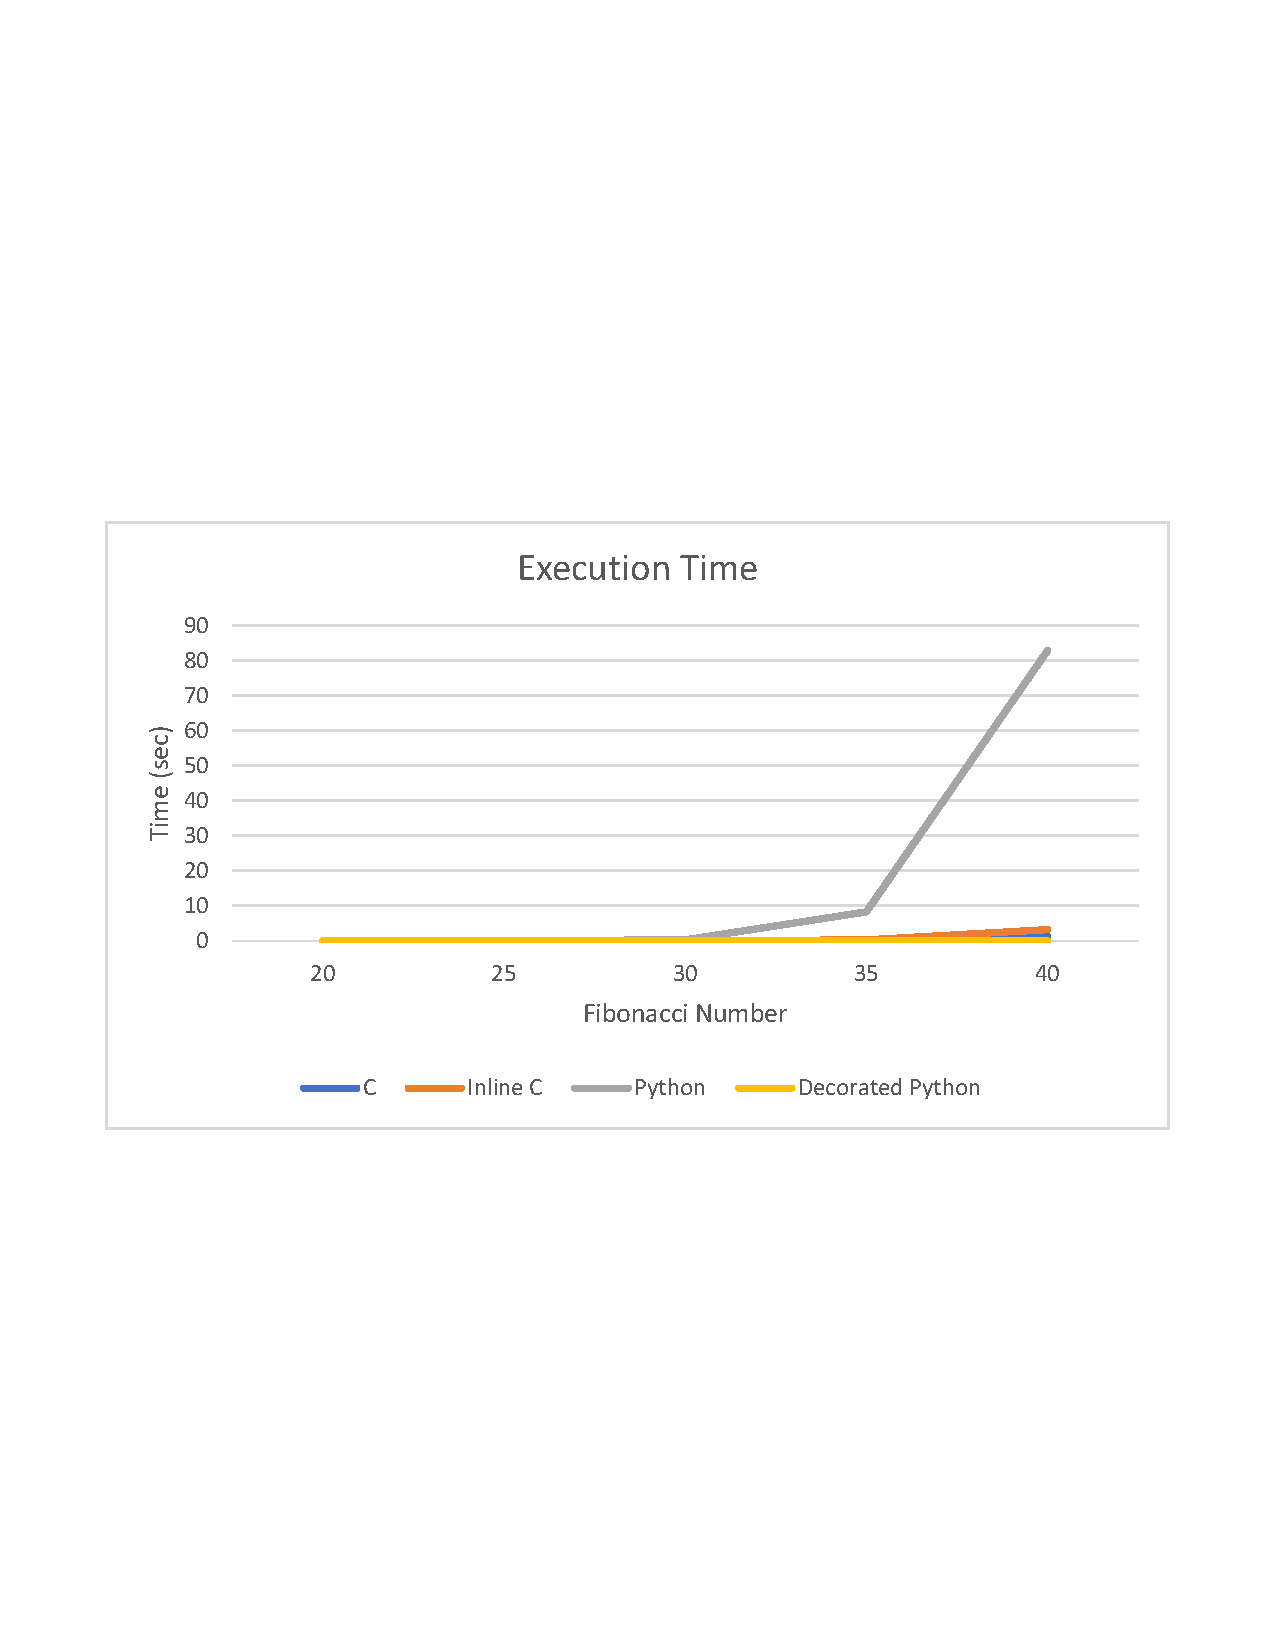
\includegraphics[width=0.47\textwidth] {ExeTime.pdf}
	\caption{Execution times for Fibonacci of 20 through 40.}
	\label{Exe Times}
\end{figure}

In Figure 1, the time exponentially increases as the Fibonacci value increments for the languages of C, Inline C, and Python. The figure depicts Python growing at the quickest speed, having a periodic growth rate of 1.18 seconds per Fibonacci Number increment. It's counterpart, Decorated Python, in possesses the slowest exponential growth at 0.015 for its periodic growth rate. C is higher at 0.69 for its periodic growth rate, and Inline C shows a periodic growth rate of 1.36. It is interesting to see an interpretted language optimized with a decorated function beating out one of the quickest compiled languages.

\begin{figure}[ht]
	\centering
		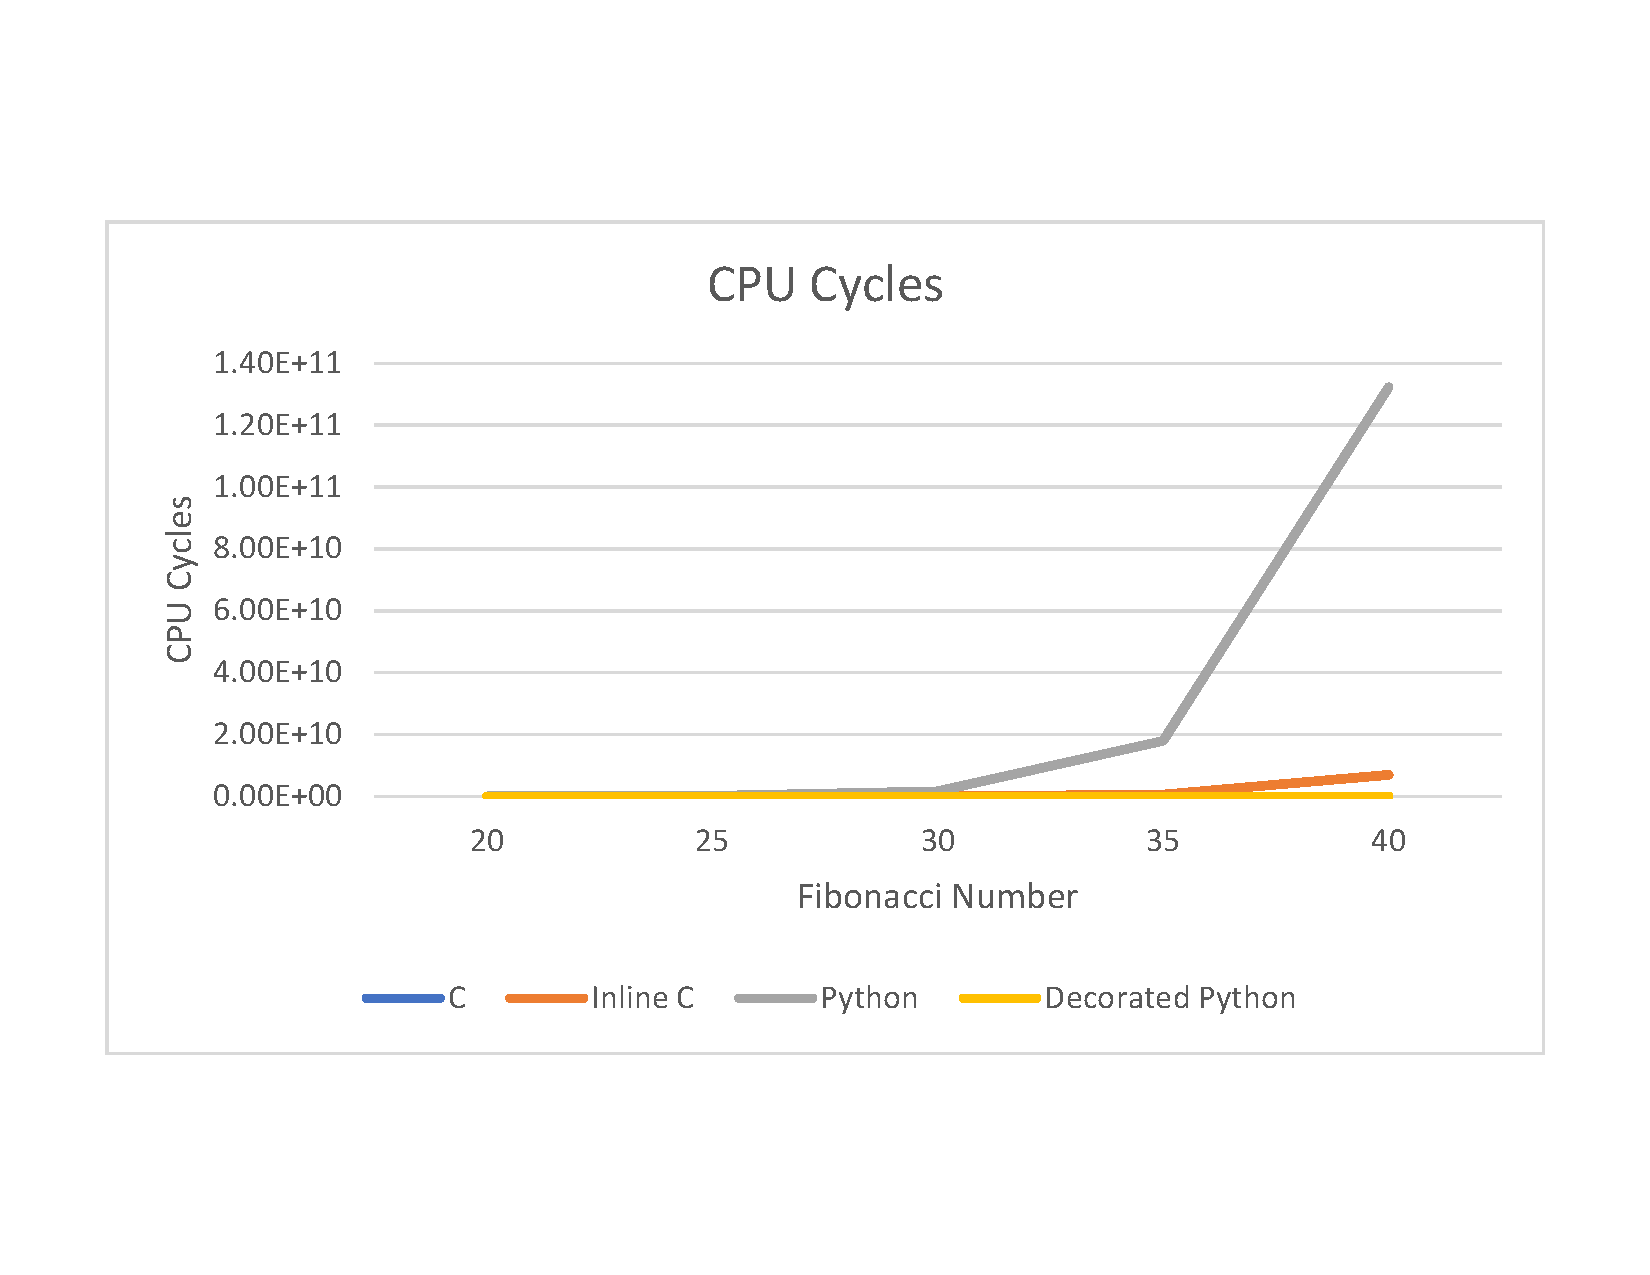
\includegraphics[width=0.47\textwidth] {CPUcycles.pdf}
	\caption{CPU cycles for Fibonacci of 20 through 40.}
	\label{CPU Cycles}
\end{figure}

Figure 2 depicts Python having the largest amount of CPU cycles used for almost every Fibonacci value tested. The number of CPU cycles reached 132,298,225,415, whereas the next highest count for Fibonacci of 40 was for Inline C, at 6,971,907,740 cycles. Clearly the optimized algorithms were not the most efficient in terms of CPU cycles.

\begin{figure}[ht]
	\centering
		\includegraphics[width=0.47\textwidth] {CacheMissesActual.pdf}
	\caption{Cache misses for Fibonacci of 20 through 40.}
	\label{Cache misses}
\end{figure}

Figure 3 shows the interpretted languages having far more cache misses than the compiled languages. Inline C had so few cache misses for Fibonacci of 20 that it didn't record the results. It is interesting to note that Decorated Python remained rather constant for its cache misses, whereas Python exponentially increased after Fibonacci of 35.

\begin{figure}[ht]
	\centering
		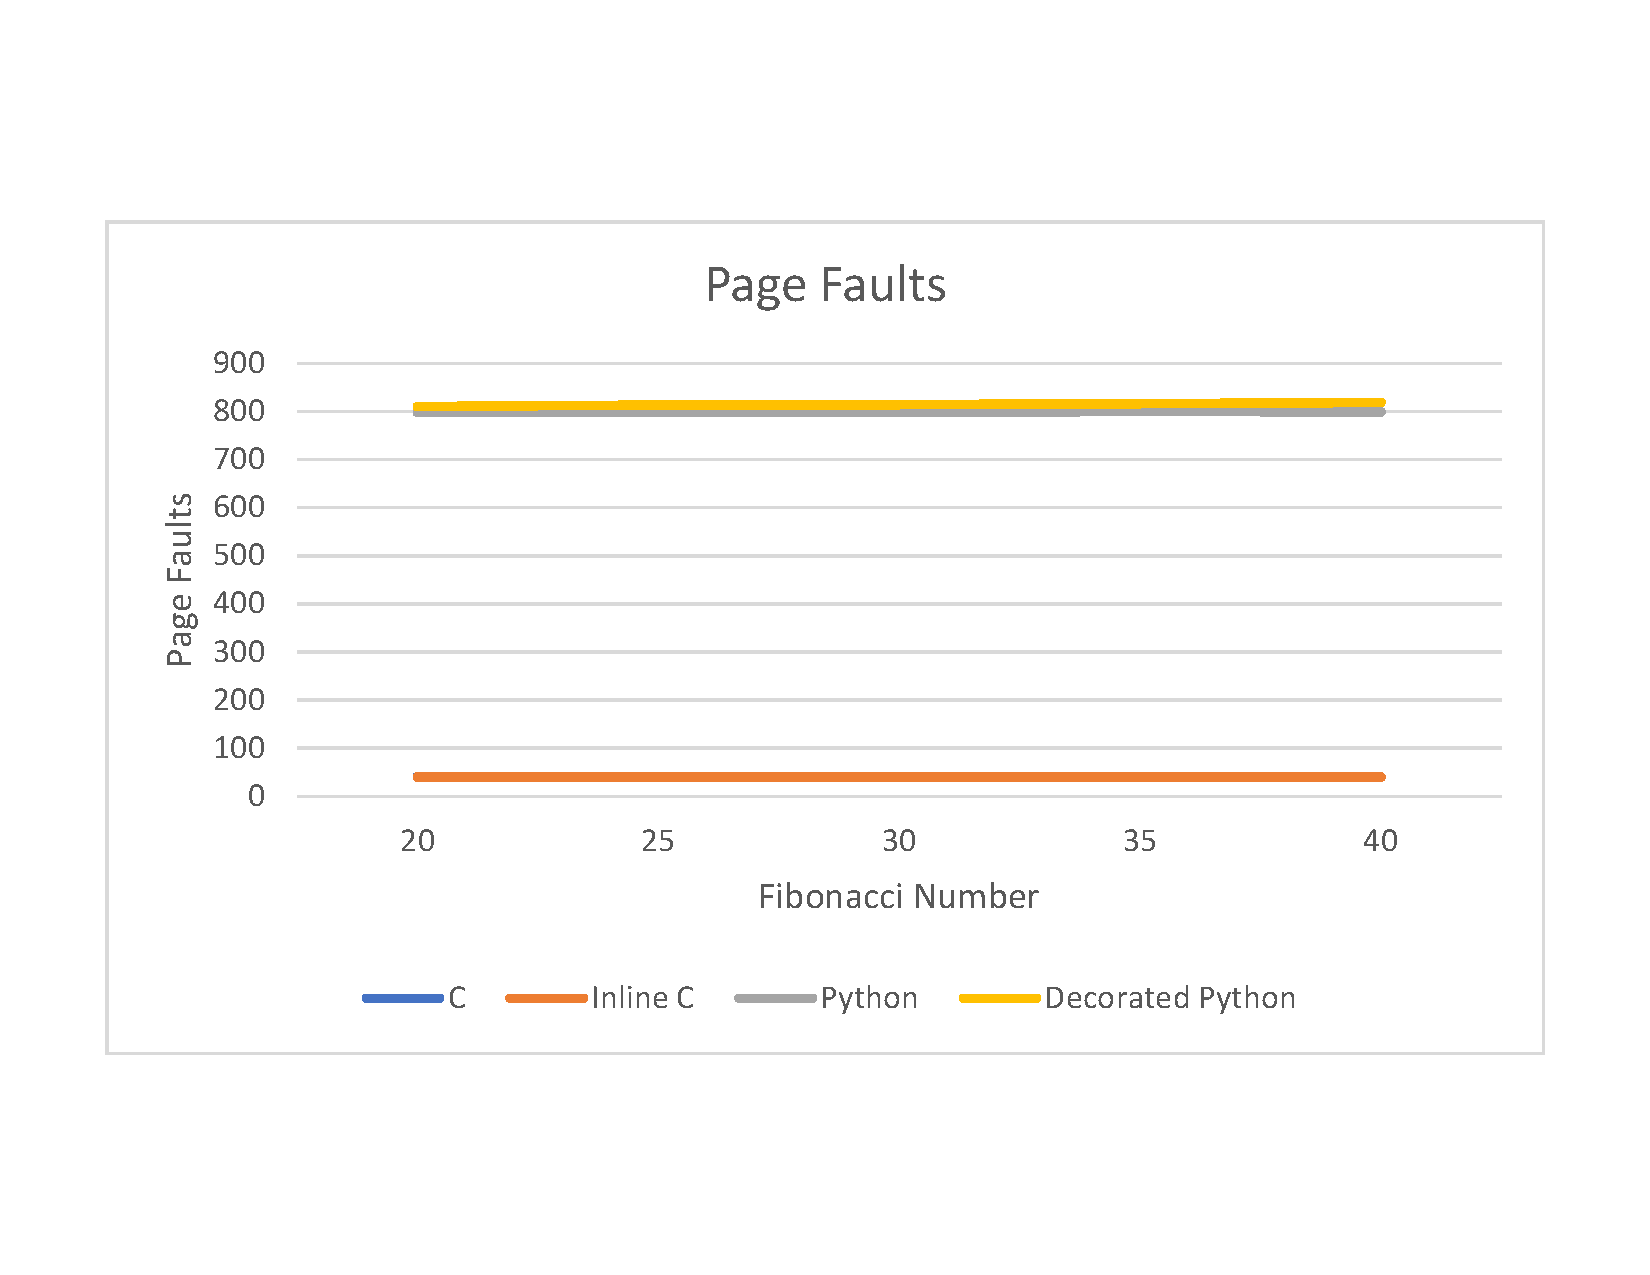
\includegraphics[width=0.47\textwidth] {PageFaults.pdf}
	\caption{Page faults for Fibonacci of 20 through 40.}
	\label{Page Faults}
\end{figure}

In Figure 4, the interpreted languages also had far more page faults than the compiled languages. Clearly the compiled languages are more efficient in terms of memory than that of the interpreted languages. The compiled algorithms didn't go over 42 page faults, whereas the interpreted languages had at least 798 page faults for each trial.

\begin{scriptsize}
\begin{table}[ht!]
  \centering
  \begin{tabular}{|l|l|}
    \hline
    \textbf{Language} & \textbf{Recursive Overhead (sec)}\\
    \hline
    C & 0.195828\\
    \hline
    Inline C & 0.852422\\
	\hline
	Python & 0.000069 \\
	\hline
	Decorated Python & 0.000082 \\
	\hline
\end{tabular}
\caption{Cost of one recursive call results for C and Python, and their corresponding optimizations.}
\label{table:formatting}
\end{table}
\end{scriptsize}

The above table indicates that the decorator function for the Python code had a higher overhead than the regular Python algorithm. However, the compiled languages were 2,388.15 times slower than the slowest interpreted algorithm. There is the potential for higher overhead with the import statements for the interpreted algorithms, but this is not the case here. In addition, since interpreted languages are executed each line at a time, the opposite results are expected here. The results do give some insight into why C and Inline C had higher execution times than the interpreted languages.

\section{Summary Statements}

It was shown that the common thought of compiled languages beating out interpretted languages in terms of execution time is not always the case; optimizations can be made to make Python a valid competitor to the compiled language of C. Even Inline C could not compete with Decorated Python when it came down to execution time. At the same time, C outperformed Python in almost every other regard. Python was much less efficient with memory allocation, resulting in more page faults and cache misses for its results. This can be due to the differences in the way that Python and C structure their memory layouts. C utilizes a stack frame, whereas Python utilizes Python objects and a private heap. Utilizing the stack is proven to be more efficient than using a heap, as a stack is trivial to allocate and deallocate memory. The heap takes longer to access due to its more complex bookkeeping of memory allocation and freeing of memory.

In addition, with many recursive calls, C would be the better choice with a faster execution time. However, inline C used far fewer CPU cycles, yet hundreds of millions more instructions than C did. When it comes down to the cache, there is little difference between Inline C and C.

Having a decorated Python function required more overhead, but it significantly improved the number of CPU cycles utilized, the number of instructions executed, and decreased the amount of cache misses. Decorated Python does take a hit with more page faults and a constant of about 15\% of all cache references being cache misses. Decorated Python outperformed C in regard to execution time, speedup, CPU cycles, clock rate, and instruction count. However, Decorated Python was far costlier in terms of page faults and cache misses.

\section{Conclusion}

Due to the massive data sets created by the Internet of Things and cloud computing, algorithmic efficiency is of the utmost importance in today's computing environment. As a response, there has been growing interest in algorithmic efficiency. In this paper we have looked at several programming languages depicting widely differing architectures, to include compiled and interpreted languages. Their performance was analyzed using the Fibonacci algorithm with Fibonacci of 20 up to Fibonacci of 50 with 5 as the increment. We have shown that while compiled languages outperform interpreted languages in almost every regard, there are optimizations that can help with certain aspects such as runtime efficiency. These improvements are important to keep in mind when considering performance efficiency of any algorithm.



%%%%%%% -- PAPER CONTENT ENDS -- %%%%%%%%


%%%%%%%%% -- BIB STYLE AND FILE -- %%%%%%%%
\bibliographystyle{ieeetr}
\bibliography{ref}
%%%%%%%%%%%%%%%%%%%%%%%%%%%%%%%%%%%%

\end{document}
